% generated by GAPDoc2LaTeX from XML source (Frank Luebeck)
\documentclass[a4paper,11pt]{report}
\usepackage[pdftex]{graphicx}
\usepackage{a4wide}
\sloppy
\pagestyle{myheadings}
\usepackage{amssymb}
\usepackage[utf8]{inputenc}
\usepackage{makeidx}
\makeindex
\usepackage{color}
\definecolor{FireBrick}{rgb}{0.5812,0.0074,0.0083}
\definecolor{RoyalBlue}{rgb}{0.0236,0.0894,0.6179}
\definecolor{RoyalGreen}{rgb}{0.0236,0.6179,0.0894}
\definecolor{RoyalRed}{rgb}{0.6179,0.0236,0.0894}
\definecolor{LightBlue}{rgb}{0.8544,0.9511,1.0000}
\definecolor{Black}{rgb}{0.0,0.0,0.0}

\definecolor{linkColor}{rgb}{0.0,0.0,0.554}
\definecolor{citeColor}{rgb}{0.0,0.0,0.554}
\definecolor{fileColor}{rgb}{0.0,0.0,0.554}
\definecolor{urlColor}{rgb}{0.0,0.0,0.554}
\definecolor{promptColor}{rgb}{0.0,0.0,0.589}
\definecolor{brkpromptColor}{rgb}{0.589,0.0,0.0}
\definecolor{gapinputColor}{rgb}{0.589,0.0,0.0}
\definecolor{gapoutputColor}{rgb}{0.0,0.0,0.0}

%%  for a long time these were red and blue by default,
%%  now black, but keep variables to overwrite
\definecolor{FuncColor}{rgb}{0.0,0.0,0.0}
%% strange name because of pdflatex bug:
\definecolor{Chapter }{rgb}{0.0,0.0,0.0}
\definecolor{DarkOlive}{rgb}{0.1047,0.2412,0.0064}


\usepackage{fancyvrb}

\usepackage{mathptmx,helvet}
\usepackage[T1]{fontenc}
\usepackage{textcomp}


\usepackage[
            pdftex=true,
            bookmarks=true,        
            a4paper=true,
            pdftitle={Written with GAPDoc},
            pdfcreator={LaTeX with hyperref package / GAPDoc},
            colorlinks=true,
            backref=page,
            breaklinks=true,
            linkcolor=linkColor,
            citecolor=citeColor,
            filecolor=fileColor,
            urlcolor=urlColor,
            pdfpagemode={UseNone}, 
           ]{hyperref}

\newcommand{\maintitlesize}{\fontsize{50}{55}\selectfont}

% write page numbers to a .pnr log file for online help
\newwrite\pagenrlog
\immediate\openout\pagenrlog =\jobname.pnr
\immediate\write\pagenrlog{PAGENRS := [}
\newcommand{\logpage}[1]{\protect\write\pagenrlog{#1, \thepage,}}
%% were never documented, give conflicts with some additional packages

\newcommand{\GAP}{\textsf{GAP}}

%% nicer description environments, allows long labels
\usepackage{enumitem}
\setdescription{style=nextline}

%% depth of toc
\setcounter{tocdepth}{1}





%% command for ColorPrompt style examples
\newcommand{\gapprompt}[1]{\color{promptColor}{\bfseries #1}}
\newcommand{\gapbrkprompt}[1]{\color{brkpromptColor}{\bfseries #1}}
\newcommand{\gapinput}[1]{\color{gapinputColor}{#1}}


\begin{document}

\logpage{[ 0, 0, 0 ]}
\begin{titlepage}
\mbox{}\vfill

\begin{center}{\maintitlesize \textbf{ Jupyter-Viz \mbox{}}}\\
\vfill

\hypersetup{pdftitle= Jupyter-Viz }
\markright{\scriptsize \mbox{}\hfill  Jupyter-Viz  \hfill\mbox{}}
{\Huge \textbf{ Jupyter Notebook Visualization Tools \mbox{}}}\\
\vfill

{\Huge  1.0.0 \mbox{}}\\[1cm]
{ 26 September 2018 \mbox{}}\\[1cm]
\mbox{}\\[2cm]
{\Large \textbf{ Nathan Carter\\
    \mbox{}}}\\
\hypersetup{pdfauthor= Nathan Carter\\
    }
\end{center}\vfill

\mbox{}\\
{\mbox{}\\
\small \noindent \textbf{ Nathan Carter\\
    }  Email: \href{mailto://ncarter@bentley.edu} {\texttt{ncarter@bentley.edu}}\\
  Homepage: \href{http://nathancarter.github.io} {\texttt{http://nathancarter.github.io}}\\
  Address: \begin{minipage}[t]{8cm}\noindent
 175 Forest St.\\
 Waltham, MA 02452\\
 USA\\
 \end{minipage}
}\\
\end{titlepage}

\newpage\setcounter{page}{2}
\newpage

\def\contentsname{Contents\logpage{[ 0, 0, 1 ]}}

\tableofcontents
\newpage

     
\chapter{\textcolor{Chapter }{How to use this package}}\label{Chapter_How_to_use_this_package}
\logpage{[ 1, 0, 0 ]}
\hyperdef{L}{X805201F27AA23554}{}
{
  

 
\section{\textcolor{Chapter }{Purpose}}\label{Section_purpose}
\logpage{[ 1, 1, 0 ]}
\hyperdef{L}{X78E0A9867DABCE86}{}
{
  

 Since 2017, it has been possible to use \textsf{GAP} in \href{http://jupyter.org/} {Jupyter} through the \textsf{JupyterKernel} package. Output was limited to the ordinary text output \textsf{GAP} produces; charts and graphs were not possible. 

 In 2018, Martins and Pfeiffer released \textsf{francy} (\href{https://github.com/mcmartins/francy} {repository}, \href{https://arxiv.org/abs/1806.08648} {article}), which lets users create graphs of a few types (vertices and edges, line
chart, bar chart, scatter chart). It also allows the user to attach actions to
the elements of these charts, which result in callbacks to \textsf{GAP} that can update the visualization. 

 This package aims to make a wider variety of visualizations accessible to \textsf{GAP} users, but does not provide tools for conveniently making such visualizations
interactive. Where the \textsf{francy} package excels at interactive visualizations, this package instead gives a
broader scope of visualization tools. 

 This is achieved by importing several existing JavaScript visualization
toolkits and exposing them to \textsf{GAP} code, as described later in this manual. 

 The toolkits currently exposed by this package are listed here. 

 
\begin{itemize}
\item  \href{https://www.anychart.com/} {AnyChart} 
\item  \href{https://canvasjs.com/} {CanvasJS} 
\item  \href{https://www.chartjs.org/} {ChartJS} 
\item  \href{http://www.cytoscape.org/} {Cytoscape} 
\item  \href{https://d3js.org/} {D3} 
\item  \href{https://plot.ly/} {Plotly} 
\item  Native HTML \texttt{canvas} element 
\item  Plain HTML 
\end{itemize}
 

 }

 
\section{\textcolor{Chapter }{Loading the package into a Jupyter notebook}}\label{Chapter_How_to_use_this_package_Section_Loading_the_package_into_a_Jupyter_notebook}
\logpage{[ 1, 2, 0 ]}
\hyperdef{L}{X80DC99A778923B3D}{}
{
  

 To import the package into a Jupyter notebook, do so just as with any other \textsf{GAP} package: Ensure that the kernel of the notebook is a \textsf{GAP} kernel, then execute the following code in one of the notebook cells. 

 
\begin{Verbatim}[commandchars=!@|,fontsize=\small,frame=single,label=Example]
  LoadPackage( "jupyter-viz" );
\end{Verbatim}
 

 }

 
\section{\textcolor{Chapter }{Creating a visualization}}\label{Chapter_How_to_use_this_package_Section_Creating_a_visualization}
\logpage{[ 1, 3, 0 ]}
\hyperdef{L}{X7878B43B78F7E099}{}
{
  

 Visualizations of any kind supported by this package are created through one
function, \texttt{CreateVisualization} (\ref{CreateVisualization}). You can view its complete documentation in for details, but examples are
given in this section. 

 Nearly all visualizations in this package are created by passing data to the \texttt{CreateVisualization} (\ref{CreateVisualization}) function as records describing what to draw. These records are converted into \href{http://www.json.org/} {JSON} form by the \textsf{json} package, and handed to whichever JavaScript toolkit you have chosen to use for
creating the visualization. 

 
\subsection{\textcolor{Chapter }{Example: AnyChart}}\label{Chapter_How_to_use_this_package_Section_Creating_a_visualization_Subsection_Example_AnyChart}
\logpage{[ 1, 3, 1 ]}
\hyperdef{L}{X7B0290B3876FCDA1}{}
{
  

 The AnyChart website contains \href{https://docs.anychart.com/Working_with_Data/Data_From_JSON} {documentation} on how to create visualizations from JSON data. Following those conventions,
we could give AnyChart the following JSON to produce a pie chart. 

 
\begin{Verbatim}[commandchars=!@|,fontsize=\small,frame=single,label=Example]
  {
      "chart" : {
          "type" : "pie",
          "data" : [
              { "x" : "Subgroups of order 6", "value" : 1 },
              { "x" : "Subgroups of order 3", "value" : 1 },
              { "x" : "Subgroups of order 2", "value" : 3 },
              { "x" : "Subgroups of order 1", "value" : 1 }
          ]
      }
  }
\end{Verbatim}
 

 In \textsf{GAP}, the same data would be represented with a record, as follows. 

 
\begin{Verbatim}[commandchars=!@|,fontsize=\small,frame=single,label=Example]
  myChartData := rec(
      chart := rec(
          type := "pie",
          data := [
              rec( x := "Subgroups of order 6", value := 1 ),
              rec( x := "Subgroups of order 3", value := 1 ),
              rec( x := "Subgroups of order 2", value := 3 ),
              rec( x := "Subgroups of order 1", value := 1 )
          ]
      )
  );
\end{Verbatim}
 

 We can ask \textsf{GAP}, running in a Jupyter notebook, to create a visualization from this data by
passing that data directly to \texttt{CreateVisualization} (\ref{CreateVisualization}). We wrap it in a record that must specify the tool to use (in this case \texttt{"anychart"}) and optionally some other details not relevant here. 

 
\begin{Verbatim}[commandchars=!@|,fontsize=\small,frame=single,label=Example]
  CreateVisualization( rec( tool := "anychart", data := myChartData ) );
\end{Verbatim}
 

 
\begin{center}
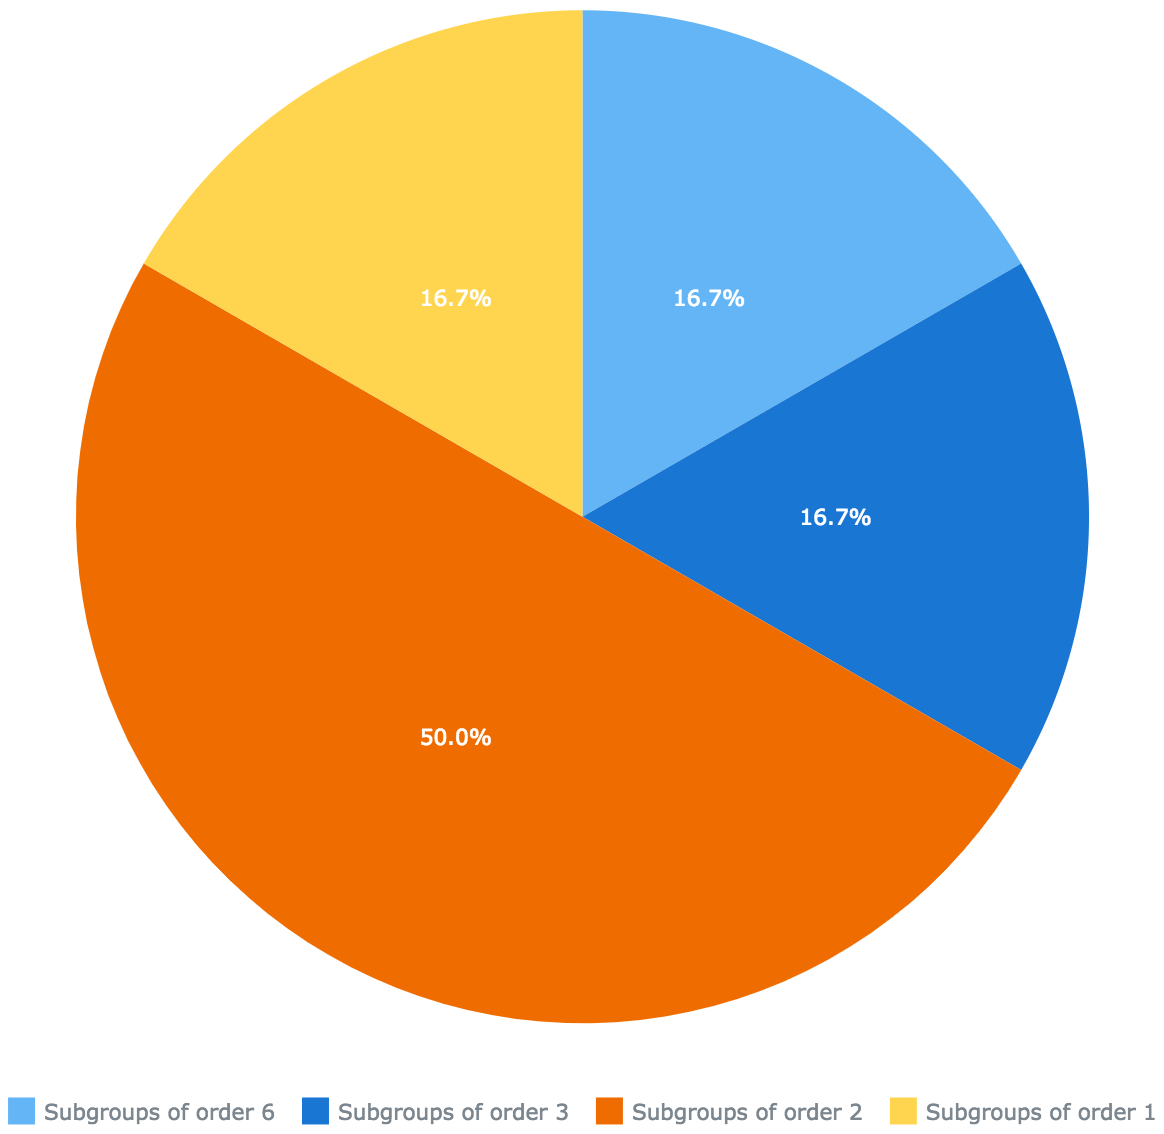
\includegraphics[width=4in]{anychart-example.png}
\end{center}
   

 If you have the data defining a visualization stored in a \texttt{.json} file on disk, you can use the following code rather than rewriting the JSON
code into \textsf{GAP} code yourself. 

 
\begin{Verbatim}[commandchars=!@|,fontsize=\small,frame=single,label=Example]
  CreateVisualization( rec(
      tool := "anychart",
      data := JsonStringToGap( ReadAll( InputTextFile( "your-file.json" ) ) )
  ) );
\end{Verbatim}
 

 AnyChart can make a wide variety of charts (area, bar, box, bubble, bullet,
column, doughnut, and so on, for over 125 different types and subtypes). Other
JavaScript libraries available also have similarly broad capabilities, but we
do not include here examples of CanvasJS, ChartJS, or Plotly, because their
capabilities and purpose are somewhat similar to that of AnyChart. Though
their data formats are different, you can find links to those formats'
documentation in the documentation for the function \texttt{CreateVisualization} (\ref{CreateVisualization}). So instead future sections focus on four other examples that are unlike
AnyChart. 

 }

 
\subsection{\textcolor{Chapter }{Post-processing visualizations}}\label{Chapter_How_to_use_this_package_Section_Creating_a_visualization_Subsection_Post-processing_visualizations}
\logpage{[ 1, 3, 2 ]}
\hyperdef{L}{X7D65933280120650}{}
{
  

 Note that \texttt{CreateVisualization} (\ref{CreateVisualization}) takes an optional second parameter, a string of JavaScript code to be run once
the visualization is complete. For example, if the visualization library did
not support a solid black border, but you wanted to add one, you could do so
in subsequent code. 

 
\begin{Verbatim}[commandchars=!@|,fontsize=\small,frame=single,label=Example]
  CreateVisualization(
      sameDataAsAbove, # plus this new second parameter:
      "visualization.style.border = '5px solid black'"
  )
\end{Verbatim}
 

 This holds for any visualization tool, not just AnyChart. In the code given in
the second parameter, two variables will be defined for your use: \texttt{element} refers to the output cell element in the notebook and \texttt{visualization} refers to the visualization that the toolkit you chose created within that
output cell (also an HTML element). 

 }

 
\subsection{\textcolor{Chapter }{Example: Cytoscape}}\label{Chapter_How_to_use_this_package_Section_Creating_a_visualization_Subsection_Example_Cytoscape}
\logpage{[ 1, 3, 3 ]}
\hyperdef{L}{X7E2737FC7EDB79B1}{}
{
  

 Unlike AnyChart, Cytoscape is for the vertices-and-edges type of graph, not
the x-and-y-axes type. A tiny Cytoscape graph (just $A\to B$) is represented by the following JSON. 

 
\begin{Verbatim}[commandchars=!@|,fontsize=\small,frame=single,label=Example]
  {
      elements : [
          { data : { id : "A" } },
          { data : { id : "B" } },
          { data : { id : "edge", source : "A", target : "B" } }
      ],
      layout : { name : "grid", rows : 1 }
  }
\end{Verbatim}
 

 Cytoscape graphs can also have style attributes not shown here. 

 Rather than copy this data directly into \textsf{GAP}, let's generate graph data in the same format using \textsf{GAP} code. Here we make a graph of the first 50 positive integers, with $n\to m$ iff $n\mid m$ (ordinary integer divisibility). 

 
\begin{Verbatim}[commandchars=!@|,fontsize=\small,frame=single,label=Example]
  N := 50;
  elements := [ ];
  roots := [ ];
  for i in [2..N] do
      Add( elements, rec( data := rec( id := String( i ) ) ) );
      if IsPrime( i ) then
          Add( roots, i );
      fi;
      for j in [2..i-1] do
          if i mod j = 0 then
              Add( elements, rec( data := rec(
                  source := String( j ),
                  target := String( i ) ) ) );
          fi;
      od;
  od;
\end{Verbatim}
 

 We then need to choose a layout algorithm. The Cytoscape documentation
suggests that the "cose" layout works well. Here, we do choose a height (in
pixels) for the result, because Cytoscape does not automaticlly resize
visualizations to fit their contents. We also set the style for each node to
display its ID (which is the integer associated with it). 

 All the code below comes directly from translating the Cytoscape documentation
from JSON form to \textsf{GAP} record form. See that documentation for more details; it is cited in the
documentation for the \texttt{CreateVisualization} (\ref{CreateVisualization}) function. 

 
\begin{Verbatim}[commandchars=!@|,fontsize=\small,frame=single,label=Example]
  CreateVisualization( rec(
      tool := "cytoscape",
      height := 600,
      data := rec(
          elements := elements, # computed in the code above
          layout := rec( name := "cose" ),
          style := [
              rec( selector := "node", style := rec( content := "data(id)" ) )
          ]
      )
  ) );
\end{Verbatim}
 

 
\begin{center}
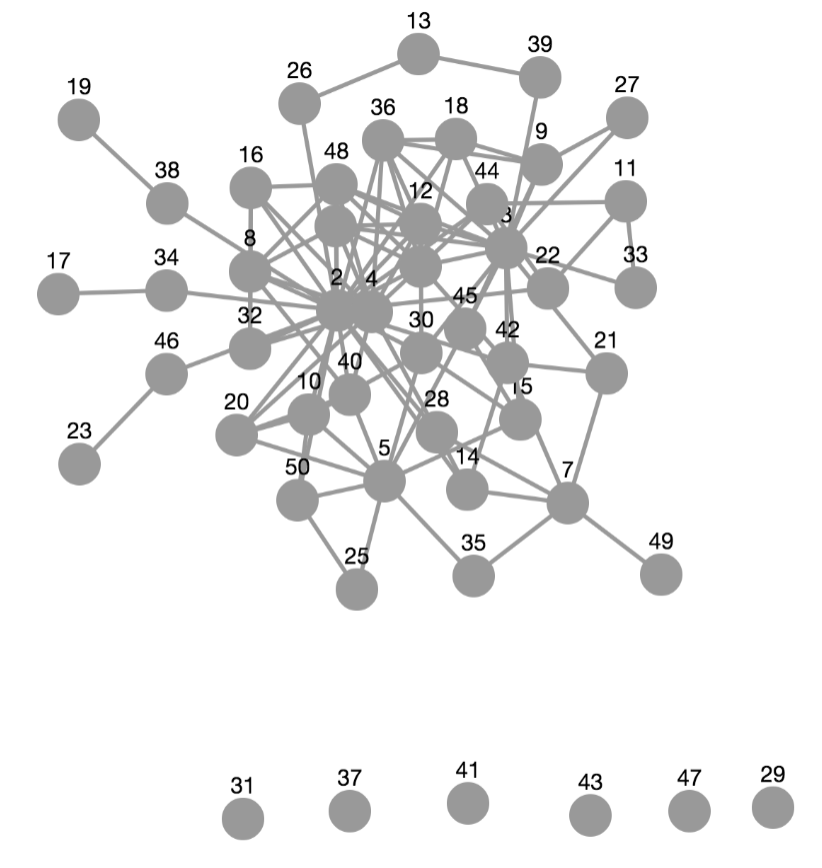
\includegraphics[width=4in]{cytoscape-example.png}
\end{center}
   

 }

 
\subsection{\textcolor{Chapter }{Example: D3}}\label{Chapter_How_to_use_this_package_Section_Creating_a_visualization_Subsection_Example_D3}
\logpage{[ 1, 3, 4 ]}
\hyperdef{L}{X7A2554B0847DD027}{}
{
  

 While D3 is one of the most famous and powerful JavaScript visualization
libraries, it does not have a JSON interface. Consequently, we can interact
with D3 only through the JavaScript code passed in the second parameter to \texttt{CreateVisualization} (\ref{CreateVisualization}). This makes it much less convenient, but we include it in this package for
those who need it. 

 
\begin{Verbatim}[commandchars=!@|,fontsize=\small,frame=single,label=Example]
  CreateVisualization(
      rec( tool := "d3" ),
      """
      // arbitrary JavaScript code can go here to interact with D3, like so:
      d3.select( visualization ).append( "circle" )
          .attr( "r", 50 ).attr( "cx", 55 ).attr( "cy", 55 )
          .style( "stroke", "red" ).style( "fill", "pink" );
      """
  );
\end{Verbatim}
 

 
\begin{center}

\includegraphics{d3-example.png}
\end{center}
   

 }

 
\subsection{\textcolor{Chapter }{Example: Native HTML Canvas}}\label{Chapter_How_to_use_this_package_Section_Creating_a_visualization_Subsection_Example_Native_HTML_Canvas}
\logpage{[ 1, 3, 5 ]}
\hyperdef{L}{X7836DDAA82B6A536}{}
{
  

 You can create a blank canvas, then use the existing JavaScript canvas API to
draw on it. 

 
\begin{Verbatim}[commandchars=!@|,fontsize=\small,frame=single,label=Example]
  CreateVisualization(
      rec( tool := "canvas", height := 300 ),
      """
      // visualization is the canvas element
      var context = visualization.getContext( '2d' );
      // draw an X
      context.moveTo( 0, 0 );
      context.lineTo( 100, 100 );
      context.moveTo( 100, 0 );
      context.lineTo( 0, 100 );
      context.stroke();
      """
  );
\end{Verbatim}
 

 
\begin{center}

\includegraphics{canvas-example.png}
\end{center}
   

 }

 
\subsection{\textcolor{Chapter }{Example: Plain HTML}}\label{Chapter_How_to_use_this_package_Section_Creating_a_visualization_Subsection_Example_Plain_HTML}
\logpage{[ 1, 3, 6 ]}
\hyperdef{L}{X7C06E0117C8EF31B}{}
{
  

 This is the degenerate example of a visualization. It does not create any
visualization, but lets you specify arbitrary HTML content instead. It is
provided here merely as a convenient way to insert HTML into the notebook. 

 
\begin{Verbatim}[commandchars=!@|,fontsize=\small,frame=single,label=Example]
  CreateVisualiation( rec(
      tool := "html",
      data := rec(
          html := "<i>Any</i> HTML can go here.  Tables, buttons, whatever."
      )
  ) );
\end{Verbatim}
 

 }

 }

 
\section{\textcolor{Chapter }{Gallery}}\label{Chapter_How_to_use_this_package_Section_Gallery}
\logpage{[ 1, 4, 0 ]}
\hyperdef{L}{X871A653B85A24E11}{}
{
  

 Readers who would like to see a gallery of examples are encouraged to inspect
the following files in this package's repository and/or installation
directory. 

 
\begin{itemize}
\item  \texttt{tst/in-noteboook-test.ipynb} shows several different visualizations, but can only be loaded in a running
Jupyter notebook with this package installed. 
\item  \texttt{tst/in-noteboook-test.pdf} is a printout, to PDF, of the previous file, with graphics included (though
printing from Jupyter notebooks is not perfect, and thus the formatting of
this PDF is not that great). 
\end{itemize}
 

 Please be aware, however, that the tools imported by this package have an
enormous breadth of capabilities not shown in that file. The reader is
encouraged to browse their websites (cited in Section \ref{Section_purpose}) for extensive galleries of visualizations. 

 
\begin{center}
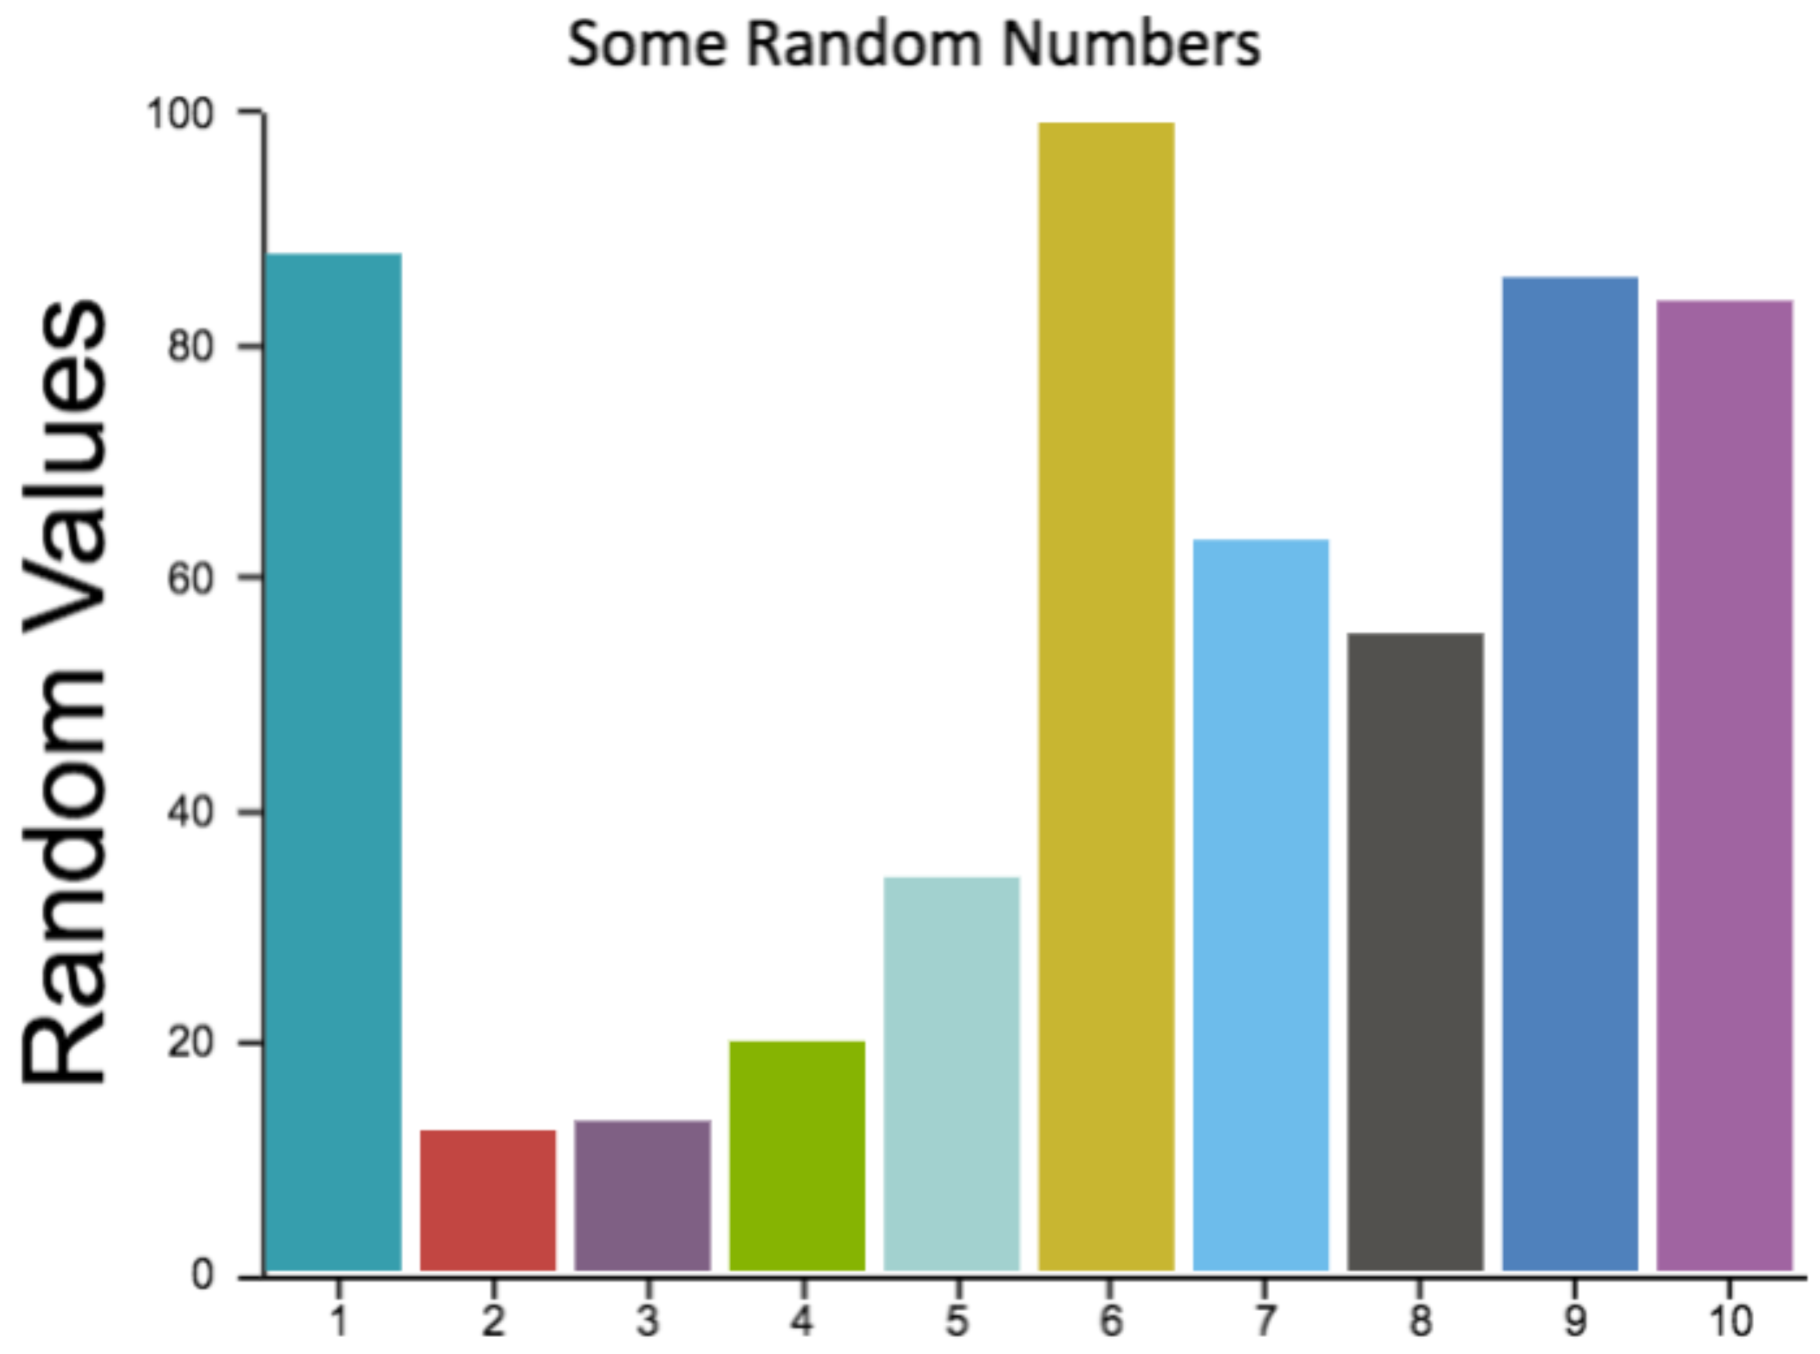
\includegraphics[width=4in]{canvasjs-example.png}
\end{center}
   

 }

 }

   
\chapter{\textcolor{Chapter }{Function reference}}\label{Chapter_Function_reference}
\logpage{[ 2, 0, 0 ]}
\hyperdef{L}{X7ECCCA82839EA283}{}
{
  
\section{\textcolor{Chapter }{Public API}}\label{Chapter_Function_reference_Section_Public_API}
\logpage{[ 2, 1, 0 ]}
\hyperdef{L}{X784AA528839119B9}{}
{
  

\subsection{\textcolor{Chapter }{RunJavaScript}}
\logpage{[ 2, 1, 1 ]}\nobreak
\hyperdef{L}{X78BDA43D7E633E33}{}
{\noindent\textcolor{FuncColor}{$\triangleright$\enspace\texttt{RunJavaScript({\mdseries\slshape script})\index{RunJavaScript@\texttt{RunJavaScript}}
\label{RunJavaScript}
}\hfill{\scriptsize (function)}}\\
\textbf{\indent Returns:\ }
an object that, if rendered in a Jupyter notebook, will run \mbox{\texttt{\mdseries\slshape script}} as JavaScript 



 If evaluated in a Jupyter notebook, its result, when rendered by that
notebook, will run the JavaScript code in \mbox{\texttt{\mdseries\slshape script}}. 

 When the given code is run, the varible \texttt{element} will be defined in its environment, and will contain the output element in the
Jupyter notebook corresponding to the code that was just evaluated. The script
is free to write to that output element. 

 This function is not intended for use in the \textsf{GAP} REPL. }

 

\subsection{\textcolor{Chapter }{LoadJavaScriptFile}}
\logpage{[ 2, 1, 2 ]}\nobreak
\hyperdef{L}{X81E2B3A07EA7A02B}{}
{\noindent\textcolor{FuncColor}{$\triangleright$\enspace\texttt{LoadJavaScriptFile({\mdseries\slshape filename})\index{LoadJavaScriptFile@\texttt{LoadJavaScriptFile}}
\label{LoadJavaScriptFile}
}\hfill{\scriptsize (function)}}\\
\textbf{\indent Returns:\ }
the string contents of the file whose name is given 



 Interprets the given \mbox{\texttt{\mdseries\slshape filename}} relative to the \texttt{lib/js/} path in the Jupyter-Viz package's installation folder, because that is where
this package stores its JavaScript libraries. A \texttt{.js} extension will be added to \mbox{\texttt{\mdseries\slshape filename}} iff needed. A \texttt{.min.js} extension will be added iff such a file exists, to prioritize minified
versions of files. 

 If the file has been loaded before in this \textsf{GAP} session, it will not be reloaded, but will be returned from a cache in memory,
for efficiency. 

 If no such file exists, returns \texttt{fail} and caches nothing. }

 

\subsection{\textcolor{Chapter }{CreateVisualization}}
\logpage{[ 2, 1, 3 ]}\nobreak
\hyperdef{L}{X7BFFD8B7808F5BDA}{}
{\noindent\textcolor{FuncColor}{$\triangleright$\enspace\texttt{CreateVisualization({\mdseries\slshape data[, code]})\index{CreateVisualization@\texttt{CreateVisualization}}
\label{CreateVisualization}
}\hfill{\scriptsize (function)}}\\
\textbf{\indent Returns:\ }
an object that, if rendered in a Jupyter notebook, will run a script to create
the desired visualization 



 The \mbox{\texttt{\mdseries\slshape data}} must be a record that will be converted to JSON using \textsf{GAP}'s \textsf{json} package. 

 The second argument is optional, a string containing JavaScript \mbox{\texttt{\mdseries\slshape code}} to run once the visualization has been created. When that code is run, the
variables \texttt{element} and \texttt{visualization} will be in its environment, the former holding the output element in the
notebook containing the visualization, and the latter holding the
visualization element itself. 

 The \mbox{\texttt{\mdseries\slshape data}} should have the following attributes. 
\begin{itemize}
\item  \texttt{tool} (required) - the name of the visualization tool to use. Currently supported
tools: 
\begin{itemize}
\item  \texttt{anychart}, whose JSON data format is given here:

 \href{https://docs.anychart.com/Working_with_Data/Data_From_JSON} {\texttt{https://docs.anychart.com/Working{\textunderscore}with{\textunderscore}Data/Data{\textunderscore}From{\textunderscore}JSON}} 
\item  \texttt{canvas}, that is, a regular HTML canvas element, on which you can draw using
arbitrary JavaScript included in the \mbox{\texttt{\mdseries\slshape code}} parameter 
\item  \texttt{canvasjs}, whose JSON data format is given here:

 \href{https://canvasjs.com/docs/charts/chart-types/} {\texttt{https://canvasjs.com/docs/charts/chart-types/}} 
\item  \texttt{chartjs}, whose JSON data format is given here:

 \href{http://www.chartjs.org/docs/latest/getting-started/usage.html} {\texttt{http://www.chartjs.org/docs/latest/getting-started/usage.html}} 
\item  \texttt{cytoscape}, whose JSON data format is given here:

 \href{http://js.cytoscape.org/#notation/elements-json} {\texttt{http://js.cytoscape.org/\#notation/elements-json}} 
\item  \texttt{d3}, which is loaded into an SVG element in the notebook's output cell, and the
caller can call any D3 methods on that element thereafter, using arbitrary
JavaScript included in the \mbox{\texttt{\mdseries\slshape code}} parameter 
\item  \texttt{html}, which fills the output element with arbitrary HTML, which the caller should
provide as a string in the \texttt{html} field of \mbox{\texttt{\mdseries\slshape data}}, as documented below 
\item  \texttt{plotly}, whose JSON data format is given here:

 \href{https://plot.ly/javascript/plotlyjs-function-reference/#plotlynewplot} {\texttt{https://plot.ly/javascript/plotlyjs-function-reference/\#plotlynewplot}} 
\end{itemize}
 
\item  \texttt{data} (required) - subobject containing all options specific to the content of the
visualization, often passed intact to the external JavaScript visualization
library. You should prepare this data in the format required by the library
specified in the \texttt{tool} field, following the documentation for that library cited above. 
\item  \texttt{width} (optional) - width to set on the output element being created 
\item  \texttt{height} (optional) - similar, but height 
\end{itemize}
 
\begin{Verbatim}[commandchars=!@|,fontsize=\small,frame=single,label=Example]
  CreateVisualization( rec(
      tool := "html",
      data := rec( html := "I am <i>SO</i> excited about this." )
  ), "console.log( 'Visualization created.' );" );
\end{Verbatim}
 }

 }

 
\section{\textcolor{Chapter }{Internal methods}}\label{Chapter_Function_reference_Section_Internal_methods}
\logpage{[ 2, 2, 0 ]}
\hyperdef{L}{X7B106BA97FD3C2BF}{}
{
  Using the convention common to \textsf{GAP} packages, we prefix all methods not intended for public use with a sequence of
characters that indicate our particular package. In this case, we use the \texttt{JUPVIZ} prefix. This is a sort of "poor man's namespacing." 

 \emph{None of these methods should need to be called by a client of this package. We
provide this documentation here for completeness, not out of necessity.} 

\subsection{\textcolor{Chapter }{JUPVIZAbsoluteJavaScriptFilename}}
\logpage{[ 2, 2, 1 ]}\nobreak
\hyperdef{L}{X7FA27984822A0E5E}{}
{\noindent\textcolor{FuncColor}{$\triangleright$\enspace\texttt{JUPVIZAbsoluteJavaScriptFilename({\mdseries\slshape filename})\index{JUPVIZAbsoluteJavaScriptFilename@\texttt{JUPVIZAbsoluteJavaScriptFilename}}
\label{JUPVIZAbsoluteJavaScriptFilename}
}\hfill{\scriptsize (function)}}\\
\textbf{\indent Returns:\ }
a JavaScript filename to an absolute path in the package dir 



 Given a relative \mbox{\texttt{\mdseries\slshape filename}}, convert it into an absolute filename by prepending the path to the \texttt{lib/js/} folder within the Jupyter-Viz package's installation folder. This is used by
functions that need to find JavaScript files stored there. 

 A \texttt{.js} extension is appended if none is included in the given \mbox{\texttt{\mdseries\slshape filename}}. }

 

\subsection{\textcolor{Chapter }{JUPVIZLoadedJavaScriptCache}}
\logpage{[ 2, 2, 2 ]}\nobreak
\hyperdef{L}{X7F877B4279081217}{}
{\noindent\textcolor{FuncColor}{$\triangleright$\enspace\texttt{JUPVIZLoadedJavaScriptCache\index{JUPVIZLoadedJavaScriptCache@\texttt{JUPVIZLoadedJavaScriptCache}}
\label{JUPVIZLoadedJavaScriptCache}
}\hfill{\scriptsize (global variable)}}\\


 A cache of the contents of any JavaScript files that have been loaded from
this package's folder. The existence of this cache means needing to go to the
filesystem for these files only once per \textsf{GAP} session. This cache is used by \texttt{LoadJavaScriptFile} (\ref{LoadJavaScriptFile}). }

 

\subsection{\textcolor{Chapter }{JUPVIZFillInJavaScriptTemplate}}
\logpage{[ 2, 2, 3 ]}\nobreak
\hyperdef{L}{X84F0A3C97FBC57EE}{}
{\noindent\textcolor{FuncColor}{$\triangleright$\enspace\texttt{JUPVIZFillInJavaScriptTemplate({\mdseries\slshape filename, dictionary})\index{JUPVIZFillInJavaScriptTemplate@\texttt{JUPVIZFillInJavaScriptTemplate}}
\label{JUPVIZFillInJavaScriptTemplate}
}\hfill{\scriptsize (function)}}\\
\textbf{\indent Returns:\ }
a string containing the contents of the given template file, filled in using
the given dictionary 



 A template file is one containing identifiers that begin with a dollar sign (\texttt{\$}). For example, \texttt{\$one} and \texttt{\$two} are both identifiers. One "fills in" the template by replacing such
identifiers with whatever text the caller associates with them. 

 This function loads the file specified by \mbox{\texttt{\mdseries\slshape filename}} by passing that argument directly to \texttt{LoadJavaScriptFile} (\ref{LoadJavaScriptFile}). If no such file exists, returns \texttt{fail}. Otherwise, it proceed as follows. 

 For each key-value pair in the given \mbox{\texttt{\mdseries\slshape dictionary}}, prefix a \texttt{\$} onto the key, suffix a newline character onto the value, and then replace all
occurrences of the new key with the new value. The resulting string is the
result. 

 The newline character is included so that if any of the values in the \mbox{\texttt{\mdseries\slshape dictionary}} contains single-line JavaScript comment characters (\texttt{//}) then they will not inadvertently affect later code in the template. }

 

\subsection{\textcolor{Chapter }{JUPVIZRunJavaScriptFromTemplate}}
\logpage{[ 2, 2, 4 ]}\nobreak
\hyperdef{L}{X8603271979CCFA2A}{}
{\noindent\textcolor{FuncColor}{$\triangleright$\enspace\texttt{JUPVIZRunJavaScriptFromTemplate({\mdseries\slshape filename, dictionary})\index{JUPVIZRunJavaScriptFromTemplate@\texttt{JUPVIZRunJavaScriptFromTemplate}}
\label{JUPVIZRunJavaScriptFromTemplate}
}\hfill{\scriptsize (function)}}\\
\textbf{\indent Returns:\ }
the composition of \texttt{RunJavaScript} (\ref{RunJavaScript}) with \texttt{JUPVIZFillInJavaScriptTemplate} (\ref{JUPVIZFillInJavaScriptTemplate}) 



 This function is quite simple, and is just a convenience function }

 

\subsection{\textcolor{Chapter }{JUPVIZRunJavaScriptUsingRunGAP}}
\logpage{[ 2, 2, 5 ]}\nobreak
\hyperdef{L}{X804379D07F29E905}{}
{\noindent\textcolor{FuncColor}{$\triangleright$\enspace\texttt{JUPVIZRunJavaScriptUsingRunGAP({\mdseries\slshape jsCode})\index{JUPVIZRunJavaScriptUsingRunGAP@\texttt{JUPVIZRunJavaScriptUsingRunGAP}}
\label{JUPVIZRunJavaScriptUsingRunGAP}
}\hfill{\scriptsize (function)}}\\
\textbf{\indent Returns:\ }
an object that, if rendered in a Jupyter notebook, will run \mbox{\texttt{\mdseries\slshape jsCode}} as JavaScript after \texttt{runGAP} has been defined 



 There is a JavaScript function called \texttt{runGAP}, defined in the \texttt{using-runGAP.js} file distributed with this package. That function makes it easy to make
callbacks from JavaScript in a Jupyter notebook to the \textsf{GAP} kernel underneath that notebook. This \textsf{GAP} function runs the given \mbox{\texttt{\mdseries\slshape jsCode}} in the notebook, but only after ensuring that \texttt{runGAP} is defined globally in that notebook, so that \mbox{\texttt{\mdseries\slshape jsCode}} can call \texttt{runGAP} as needed. 

 Here is an example use, from JavaScript, of the \texttt{runGAP} function. 
\begin{Verbatim}[commandchars=!@|,fontsize=\small,frame=single,label=Example]
  var calculation = "2^50";
  runGAP( calculation + ";", function ( result, error ) {
      if ( result )
          alert( calculation + "=" + result );
      else
          alert( "There was an error: " + error );
  } );
\end{Verbatim}
 }

 

\subsection{\textcolor{Chapter }{JUPVIZRunJavaScriptUsingLibraries}}
\logpage{[ 2, 2, 6 ]}\nobreak
\hyperdef{L}{X79B7692C7F543161}{}
{\noindent\textcolor{FuncColor}{$\triangleright$\enspace\texttt{JUPVIZRunJavaScriptUsingLibraries({\mdseries\slshape libraries, jsCode})\index{JUPVIZRunJavaScriptUsingLibraries@\texttt{JUPVIZRunJavaScriptUsingLibraries}}
\label{JUPVIZRunJavaScriptUsingLibraries}
}\hfill{\scriptsize (function)}}\\
\textbf{\indent Returns:\ }
an object that, if rendered in a Jupyter notebook, will run \mbox{\texttt{\mdseries\slshape jsCode}} as JavaScript after all \mbox{\texttt{\mdseries\slshape libraries}} have been loaded 



 There are a set of JavaScript libraries stored in the \texttt{lib/js/} subfolder of this package's installation folder. The Jupyter notebook does
not, by default, know about any of those libraries. This \textsf{GAP} function runs the given \mbox{\texttt{\mdseries\slshape jsCode}} in the notebook, but only after ensuring that all JavaScript files on the list \mbox{\texttt{\mdseries\slshape libraries}} have been loaded, so that \mbox{\texttt{\mdseries\slshape jsCode}} can make use of the functions and variables that they define. 

 If the first parameter is given as a string instead of a list of strings, it
is treated as a list of just one string. 
\begin{Verbatim}[commandchars=!@|,fontsize=\small,frame=single,label=Example]
  JUPVIZRunJavaScriptUsingLibraries( [ "mylib.js" ],
      "alert( 'My Lib defines foo to be: ' + window.foo );" );
  # Equivalently:
  JUPVIZRunJavaScriptUsingLibraries( "mylib.js",
      "alert( 'My Lib defines foo to be: ' + window.foo );" );
\end{Verbatim}
 }

 }

 
\section{\textcolor{Chapter }{Representation wrapper}}\label{Chapter_Function_reference_Section_Representation_wrapper}
\logpage{[ 2, 3, 0 ]}
\hyperdef{L}{X7CB82ABE7B3255EB}{}
{
  This code is documented for completeness's sake only. It is not needed for
clients of this package. Package maintainers may be interested in it in the
future. 

 The \textsf{JupyterKernel} package defines a method \texttt{JupyterRender} that determines how \textsf{GAP} data will be shown to the user in the Jupyter notebook interface. When there
is no method implemented for a specific data type, the fallback method uses
the built-in \textsf{GAP} method \texttt{ViewString}. 

 This presents a problem, because we are often transmitting string data (the
contents of JavaScript files) from the \textsf{GAP} kernel to the notebook, and \texttt{ViewString} is not careful about how it escapes characters such as quotation marks, which
can seriously mangle code. Thus we must define our own type and \texttt{JupyterRender} method for that type, to prevent the use of \texttt{ViewString}. 

 The declarations documented below do just that. In the event that \texttt{ViewString} were upgraded to more useful behavior, this workaround could probably be
removed. Note that it is used explicitly in the \texttt{using-library.js} file in this package. 

\subsection{\textcolor{Chapter }{JUPVIZIsFileContents (for IsObject)}}
\logpage{[ 2, 3, 1 ]}\nobreak
\hyperdef{L}{X82269732822D224D}{}
{\noindent\textcolor{FuncColor}{$\triangleright$\enspace\texttt{JUPVIZIsFileContents({\mdseries\slshape arg})\index{JUPVIZIsFileContents@\texttt{JUPVIZIsFileContents}!for IsObject}
\label{JUPVIZIsFileContents:for IsObject}
}\hfill{\scriptsize (filter)}}\\
\textbf{\indent Returns:\ }
\texttt{true} or \texttt{false} 



 The type we create is called \texttt{FileContents}, because that is our purpose for it (to preserve, unaltered, the contents of
a text file). }

 

\subsection{\textcolor{Chapter }{JUPVIZIsFileContentsRep (for IsComponentObjectRep and JUPVIZIsFileContents)}}
\logpage{[ 2, 3, 2 ]}\nobreak
\hyperdef{L}{X84D70ACD7A72AA84}{}
{\noindent\textcolor{FuncColor}{$\triangleright$\enspace\texttt{JUPVIZIsFileContentsRep({\mdseries\slshape arg})\index{JUPVIZIsFileContentsRep@\texttt{JUPVIZIsFileContentsRep}!for IsComponentObjectRep and JUPVIZIsFileContents}
\label{JUPVIZIsFileContentsRep:for IsComponentObjectRep and JUPVIZIsFileContents}
}\hfill{\scriptsize (filter)}}\\
\textbf{\indent Returns:\ }
\texttt{true} or \texttt{false} 



 The representation for the \texttt{FileContents} type }

 

\subsection{\textcolor{Chapter }{JUPVIZFileContents (for IsString)}}
\logpage{[ 2, 3, 3 ]}\nobreak
\hyperdef{L}{X7D401DB582A5EBA2}{}
{\noindent\textcolor{FuncColor}{$\triangleright$\enspace\texttt{JUPVIZFileContents({\mdseries\slshape arg})\index{JUPVIZFileContents@\texttt{JUPVIZFileContents}!for IsString}
\label{JUPVIZFileContents:for IsString}
}\hfill{\scriptsize (operation)}}\\


 A constructor for \texttt{FileContents} objects }

 Elsewhere, the \textsf{Jupyter-Viz} package also installs a \texttt{JupyterRender} method for \texttt{FileContents} objects that just returns their text content untouched. }

 }

   
\chapter{\textcolor{Chapter }{Adding new visualization tools}}\label{Chapter_Adding_new_visualization_tools}
\logpage{[ 3, 0, 0 ]}
\hyperdef{L}{X81249ADA79916213}{}
{
  

 
\section{\textcolor{Chapter }{Why you might want to do this}}\label{Chapter_Adding_new_visualization_tools_Section_Why_you_might_want_to_do_this}
\logpage{[ 3, 1, 0 ]}
\hyperdef{L}{X7DB91A9C7C03FF67}{}
{
  

 The visualization tools made available by this package (Plotly, D3, CanvasJS,
etc.) provide many visualization options. However, you may come across a
situation that they do not cover. Or a new and better tool may be invented
after this package is created, and you wish to add it to the package. 

 Currently, the only supported way to do this is to alter the package code
itself. In the future, it would be nice to make it so that you can register
new visualization tools with the package without modifying the package code.
But until then, this is the supported method. 

 }

 
\section{\textcolor{Chapter }{What you will need}}\label{Chapter_Adding_new_visualization_tools_Section_What_you_will_need}
\logpage{[ 3, 2, 0 ]}
\hyperdef{L}{X858B113D80E8D32B}{}
{
  

 Before proceeding, you will need the following information: 
\begin{itemize}
\item  A URL on the internet that serves the JavaScript code defining the new
visualization tool you wish to add. For instance, the ChartJS library is
imported from CloudFlare, at \href{https://cdnjs.cloudflare.com/ajax/libs/Chart.js/2.7.2/Chart.bundle.min} {\texttt{https://cdnjs.cloudflare.com/ajax/libs/Chart.js/2.7.2/Chart.bundle.min}}. It is best if you have this URL from a Content Delivery Network (CDN) to
ensure very high availability. 
\item  Knowledge of how to write a short JavaScript function that can embed the given
tool into any given DOM \texttt{Element}. For many tools, this is just a single call to the main class's contructor or
the library's initialization function. 
\item  While not necessary, it makes things easy if you know what function to call in
your chosen library to define a visualization from JSON data. This makes it
easier for users to pass all the required data and options from \textsf{GAP} code, which is the typical user's preferred way of defining a visualization. 
\end{itemize}
 

 }

 
\section{\textcolor{Chapter }{The appropriate procedure}}\label{Chapter_Adding_new_visualization_tools_Section_The_appropriate_procedure}
\logpage{[ 3, 3, 0 ]}
\hyperdef{L}{X8251958E7CD211DE}{}
{
  

 Throughout these steps, I will assume that the name of the new tool you wish
to install is \texttt{NEWTOOL}. I choose all capital letters to make it stand out, so that you can tell
where you need to fill in blanks in the examples, but you should probably use
lower-case letters, to match the convention used by all of the built-in tools. 

 
\begin{enumerate}
\item Clone the repository for this package.
\item Enter the \texttt{lib/js/} folder in the repository.
\item Duplicate the file \texttt{viz-tool-chartjs.js} and rename it suitably for the tool you wish to import, such as \texttt{viz-tool-NEWTOOL.js}. It \emph{must} begin with \texttt{viz-tool-}.
\item Edit that file. At the top, you will notice the installation of the CDN URL
mentioned in the previous section. Replace it with the URL for your toolkit,
and replace the identifier \texttt{chartjs} with \texttt{NEWTOOL}. 
\begin{Verbatim}[commandchars=!@|,fontsize=\small,frame=single,label=Example]
  window.requirejs.config( {
      paths : {
          NEWTOOL : 'https://cdn.example.com/NEWTOOL.min.js'
      }
  } );
\end{Verbatim}
 
\item In the middle of the same file, feel free to update the comments to reflect
your toolkit rather than ChartJS.
\item At the end of the same file, you will notice code that installs \texttt{chartjs} as a new function in the \texttt{window.VisualizationTools} object. Replace it with code that installs your tool instead. See the comments
below for some guidance. 
\begin{Verbatim}[commandchars=!@|,fontsize=\small,frame=single,label=Example]
  window.VisualizationTools.NEWTOOL = function ( element, json, callback ) {
      // The variable "element" is the output cell in the notebook into
      // which you should place your visualization.  For example, perhaps
      // your new toolkit draws in SVG elements, so you need one:
      var result = document.createElement( 'SVG' );
      element.append( result );
      // The variable "json" is all the data, in JSON form, passed from
      // GAP to tell you how to create a visualization.  The data format
      // convention is up to you to explain and document with your new
      // tool.  Two attributes in particular are important here, "width"
      // and "height" -- if you ignore everything else, at least respect
      // those in whatever way makes sense for your visualization.  Here
      // is an example for an SVG:
      if ( json.width ) result.width = json.width;
      if ( json.height ) result.width = json.height;
      // Then use RequireJS to import your toolkit (which will use the CDN
      // URL you registered above) and use it to fill the element with the
      // desired visualization.  You may or may not need to modify "json"
      // before passing it to your toolkit; this is up to the conventions
      // you choose to establish.
      require( [ 'NEWTOOL' ], function ( NEWTOOL ) {
          // Use your library to set up a visualization.  Example:
          var viz = NEWTOOL.setUpVisualizationInElement( result );
          // Tell your library what to draw.  Example:
          viz.buildVisualizationFromJSON( json );
          // Call the callback when you're done.  Pass the element you were
          // given, plus the visualization you created.
          callback( element, result );
      } );
  };
\end{Verbatim}
 
\item Optionally, in the \texttt{lib/js/} folder, run the \texttt{minify-all-scripts.sh} script, which compresses your JavaScript code to save on data transfer, memory
allocation, and parsing time. Rerun that script each time you change your file
as well.
\item You should now be able to use your new visualization tool in \textsf{GAP}. Verify that your changes worked, and debug as necessary. You may be able to
notice the change only if you refresh in your browser the page containing the
Jupyter notebook in question and also restart the \textsf{GAP} kernel in that same page. Then try code like the following in the Jupyter
notebook to test what you've done. 
\begin{Verbatim}[commandchars=!@|,fontsize=\small,frame=single,label=Example]
  CreateVisualization( rec(
      tool := "NEWTOOL",
      # any other data you need goes here
  ) );
\end{Verbatim}
 
\item Once your changes work, commit them to the repository and submit a pull
request back to the original repository, to have your work included in the
default distribution.
\end{enumerate}
 A complete and working (but silly) example follows. This portion would go in \texttt{lib/js/viz-tool-color.js}: 
\begin{Verbatim}[commandchars=!@|,fontsize=\small,frame=single,label=Example]
  // No need to import any library from a CDN for this baby example.
  window.VisualizationTools.color = function ( element, json, callback ) {
      // just writes json.text in json.color, that's all
      var span = document.createElement( 'span' );
      span.textContent = json.text;
      span.style.color = json.color;
      callback( element, span );
  };
\end{Verbatim}
 

 This is an example usage of that simple tool from \textsf{GAP} in a Jupyter notebook: 

 
\begin{Verbatim}[commandchars=!@|,fontsize=\small,frame=single,label=Example]
  CreateVisualization( rec(
      tool := "color",
      text := "Happy St. Patrick's Day.",
      color := "green"
  ) );
\end{Verbatim}
 

 }

 }

 \def\indexname{Index\logpage{[ "Ind", 0, 0 ]}
\hyperdef{L}{X83A0356F839C696F}{}
}

\cleardoublepage
\phantomsection
\addcontentsline{toc}{chapter}{Index}


\printindex

\immediate\write\pagenrlog{["Ind", 0, 0], \arabic{page},}
\newpage
\immediate\write\pagenrlog{["End"], \arabic{page}];}
\immediate\closeout\pagenrlog
\end{document}
